\documentclass[11pt,a4paper]{scrreprt}
\usepackage{graphicx}
\usepackage[ngerman]{babel} 
\usepackage[T1]{fontenc}
\usepackage[utf8]{inputenc} 
\usepackage{setspace}
\usepackage{tabularx}
\usepackage{wrapfig}
\usepackage{acronym}
\usepackage{hyperref}
\usepackage{color}
\usepackage[a4paper,left=2cm,right=2cm,top=3cm,bottom=3cm]{geometry}
\usepackage{float}
\usepackage{listings}
\lstset{literate=%
    {Ö}{{\"O}}1
    {Ä}{{\"A}}1
    {Ü}{{\"U}}1
    {ß}{{\ss}}1
    {ü}{{\"u}}1
    {ä}{{\"a}}1
    {ö}{{\"o}}1
    {~}{{\textasciitilde}}1
}
\usepackage{pdfpages}
\usepackage[headsepline,footsepline]{scrlayer-scrpage}
\renewcommand*{\chapterheadstartvskip}{\vspace*{0.0\baselineskip}}
\renewcommand{\chapterpagestyle}{scrheadings}
\pagestyle{scrheadings}
\clearscrheadfoot
\ihead{\headmark}
\ohead{\pagemark}
\ifoot{Benjamin Mosberger, Tobias Schoch}
\automark{chapter}
\setkomafont{subparagraph}{\normalfont\itshape}
\RedeclareSectionCommand[beforeskip=-.5\baselineskip, afterskip=-1em]{subparagraph}


%--------Titelseite----------
\KOMAoptions{fontsize=12pt}
\begin{document}
\newgeometry{left=0cm,right=0cm, top=1cm} 
\thispagestyle{empty}
\begin{center}
	
\includegraphics[height=2cm]{./Bilder/logo_ntb.png}
	\hspace*{3cm}
	
\includegraphics[height=1.6cm]{./Bilder/logo_htw.png}\\
	\vspace{3cm}
	\Large{NTB - Interstaatliche Hochschule für Technik Buchs}\\
	\vspace{4cm}
	\textbf{IuK\_IV}\\
	\textbf{Semesterprojekt Webapplikation}\\
	\vspace{6cm}
	\large{}
	\doublespacing
	\begin{tabular}{ll}
		\textbf{Studierende:} & Mosberger Benjamin, \href{mailto:benjamin.mosberger@ntb.ch}{benjamin.mosberger@ntb.ch}\\ 
		& Tobias Schoch, \href{mailto:tobias.schoch@ntb.ch}{tobias.schoch@ntb.ch}\\ 
		\textbf{Referent:} & Studer Martin, \href{mailto: martin.studer@htwchur.ch}{martin.studer@htwchur.ch} \\
		\textbf{Datum:} & FS 2016
	\end{tabular}
\end{center}
\KOMAoptions{fontsize=11pt}
\restoregeometry
\pagebreak


%--------Inhaltsverzeichnis---------- 
\tableofcontents 
\pagebreak

%%--------listings----------
%\lstlistoflistings
%\newpage

%--------Inhalt----------
\chapter{Projektidee}
Ein Webtool zur Suche von Ersatzteilen oder Dienstleistungen im Zusammenhang mit Autos soll erstellt werden. Dabei soll der Benutzer sich mit Facebook einloggen können, um allfällige Bewertungen abzugeben. Das Facebook-Login verhindert, dass eine Person zu viele gute oder schlechte Bewertungen verteilt. Der Benutzer kann nun eine Postleitzahl, eine maximale Reichweite und Stichwörter eingeben, daraus wird dem Benutzer eine Liste mit den verschiedenen Anbietern angezeigt mit einer kurzen Beschreibung, durch anklicken wird das komplette Profil des Anbieters angezeigt und es kann Kontakt aufgenommen werden. Die Liste der Anbieter Dienstleistungen sollen sich ebenfalls mit Facebook einloggen können und durch Anwählen eines Buttons zum Backend der Webapp gelangen, wo Sie Ihre Daten selber eingeben können. Es soll auch möglich sein, Fotos Ihrer Arbeiten zur Vorschau zur Verfügung zu stellen. 

\chapter{Projektskizze}
\textbf{Ziel:}\\
Mit dem Dienstleistungsportal soll dem Nutzer die Suche nach geeigneten Anbietern im Automobilbereich in der näheren Umgebung massgeblich vereinfacht werden. Im Vergleich zu heute,wo die Suche hauptsächlich über Facebook und Empfehlungen von Fremden stattfindet soll ausserdem ein seriöses Bewertungssystem eingeführt werden.\\

\noindent
\textbf{Umsetzung:}\\
Die Webapplikation soll mit Bootstrap erstellt werden. Zum Einloggen soll der Facebook-Account verwendet werden. Damit wird auch das Bewertungssystem der Anbieter überwacht, jeder Nutzer soll einen Anbieter nur maximal 1 mal bewerten können. Likes sollen auf dieser Plattform keinen Stellenwert haben.\\

\noindent
\textbf{Laufzeit:}\\
Das Projekt erstreckt sich über das Frühlingssemester 2016. Das Abgabedatum ist der 03.06.2016.\\

\noindent
\textbf{Finanzierung:}\\
Das Projekt soll finanzielle Mittel auskommen. Es sind lediglich 60 Arbeitsstunden pro Student gerechnet.

\chapter{Anforderungsdokumentation}
\section{Anforderungsliste}
\begin{tabular}{ll}
    A.1 & Der Kunde kann sich mit dem Facebook Account anmelden\\
    A.2 & Der Dienstleister erstellt einen neuen Account\\
    A.3 & Der Dienstleister kann sein Profil editieren\\
    A.4 & Der Kunde kann nach Dienstleistung suchen\\
    A.5 & Der Kunde kann nach Radius suchen\\
    A.6 & Der Kunde kann den Dienstleister mit 1-5 bewerten\\
    A.7 & Der Kunde kann zwischen den Ansichten Liste und Map wählen\\
    A.8 & Der Dienstleister kann 0-3 Bilder hoch laden\\
    A.9 & Der Dienstleister kann 1-n Dienstleistungen angeben\\

\end{tabular}\\

\newpage
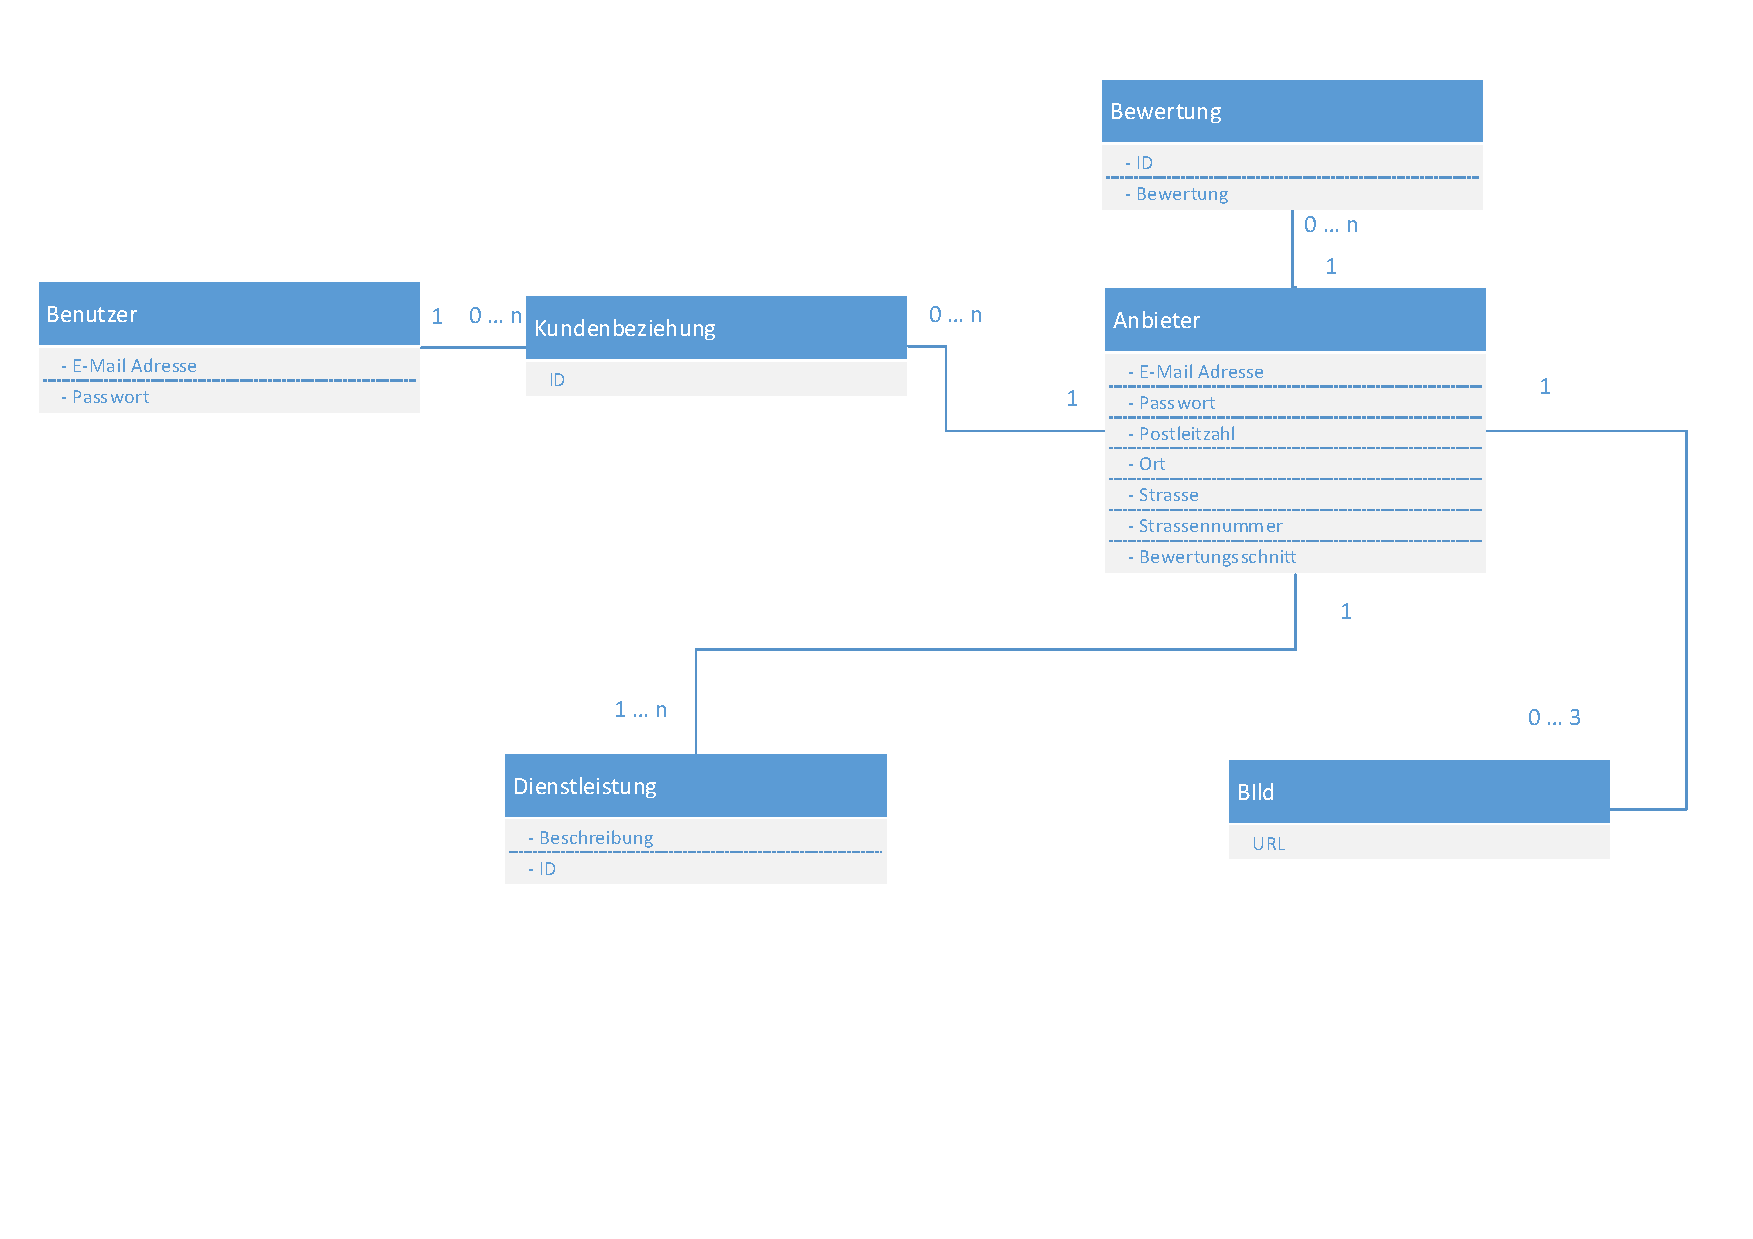
\includepdf[scale=0.7, pages=-, angle=90,pagecommand=\section{Datenmodell} \thispagestyle{headings}]{./Bilder/Datenmodell.pdf} 


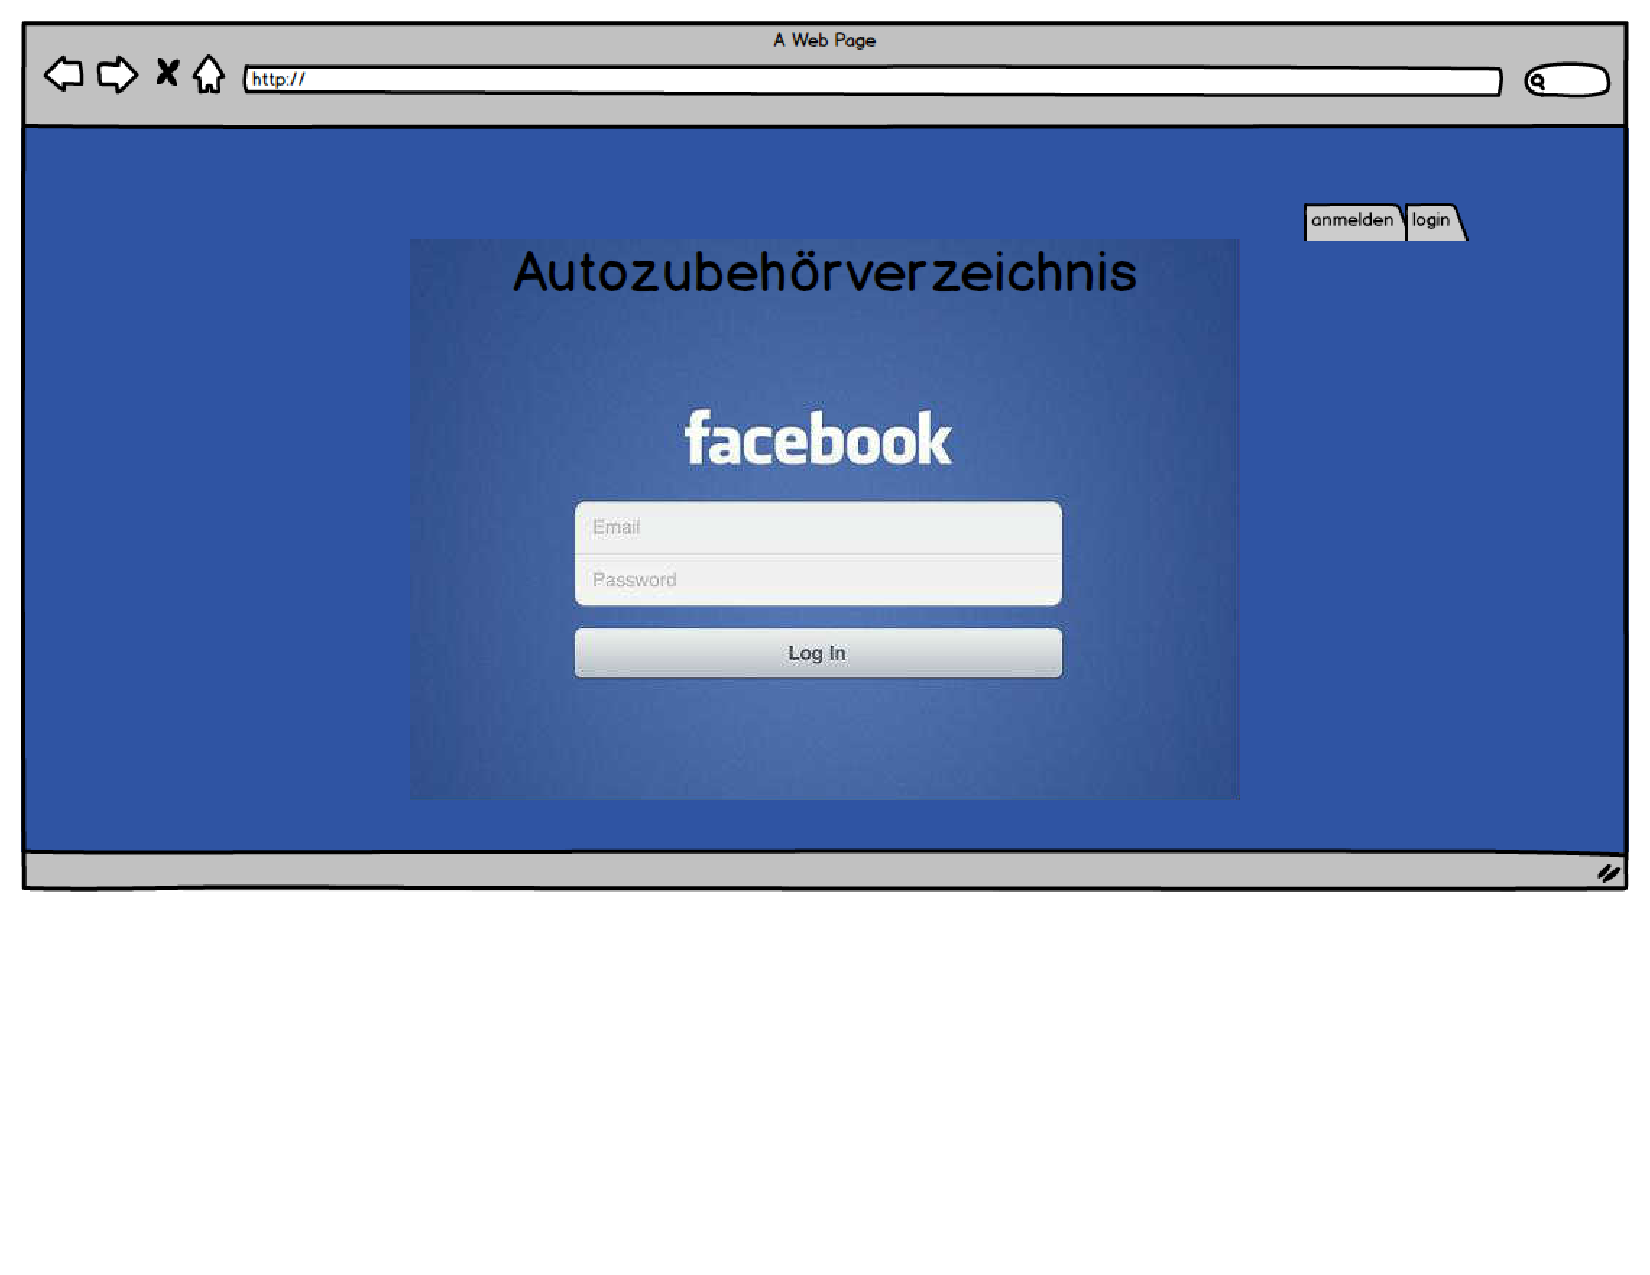
\includepdf[scale=0.75, pages=1-2, nup=1x2, angle=0,pagecommand=\section{Mockup} \thispagestyle{headings} ]{./Bilder/mockup.pdf} 
\includepdf[scale=0.75, pages=3-, nup=1x2, angle=0,pagecommand= \thispagestyle{headings} ]{./Bilder/mockup.pdf} 

\chapter{Architektur}
GitHub-Repo: \url{https://github.com/tschoch/webapplikation}
\section{Allgemein}


\section{Facebook Login}
Facebook login mit PHP SDK \cite{phpsdk}.

\begin{lstlisting}[language=PHP, frame=single, captionpos=b,caption= search\_list.php]

//session start
<?php
session_start(); 
?>

//prüfe ob eingeloggt
<?php if ($_SESSION['FBID']):
...
php else: 
...
php endif 
?> 
\end{lstlisting}

\noindent
zugriff auf variablen:
\begin{lstlisting}[language=PHP, frame=single, captionpos=b,caption= fbconfig.php]
 // 
 $graphObject = $response->getGraphObject();
  
         // speichere Facebookvariablen (id,name,email)
         $fbid = $graphObject->getProperty('id');
         $fbfullname = $graphObject->getProperty('name');
         $femail = $graphObject->getProperty('email');
         
         //speichere Werte in Sessionvariablen
         $_SESSION['FBID'] = $fbid;
         $_SESSION['FULLNAME'] = $fbfullname;
         $_SESSION['EMAIL'] =  $femail;
 	    
\end{lstlisting}

\newpage
\section{Maps}

\newpage
\begin{thebibliography}{999}

\bibitem{phpsdk}  Github. facebook-php-sdk-v4
 URL: \url{https://github.com/facebook/facebook-php-sdk-v4/} [Stand 6.4.2016].
\end{thebibliography}
\end{document}









